\section{Spatial-econometric diagnostics}
\label{app:spatial}

\subsection{Question and weight matrices}
The spatial analysis asks whether countries with similar version changes are geographic
neighbors and whether the mean contrasts survive spatial dependence. It does not estimate
cultural diffusion, policy spillovers, or a temporal model. Coordinates are pinned to
the versioned roster and Natural Earth \citep{naturalearth}. The primary matrix is a
symmetric four-nearest-neighbor graph based on great-circle distance and row-standardized
after symmetrization; $k=6,8$ are robustness checks.

\subsection{Global diagnostics}
Moran's $I$ evaluates spatial covariance \citep{moran1950notes}; Geary's $C$ emphasizes
squared local differences \citep{geary1954contiguity}. Each uses 9,999 random
permutations and a plus-one two-sided Monte Carlo $p$-value. Benjamini--Hochberg
adjustment spans 27 primary $k=4$ outcomes: nine outcomes for GPT-5.5, GPT-5.6 Sol, and
their contrast. The CRG version contrast gives Moran $I=0.225$ ($q=0.059$) and Geary
$C=0.752$ ($q=0.032$); only Geary's local-difference signal crosses the corrected 5\%
threshold. The global TVD contrast is not significantly clustered after this correction.

\subsection{Spatial-error and spatial-HAC sensitivity}
For a country-level contrast $y$, the maximum-likelihood spatial-error model is
\[
y=\alpha\mathbf 1+u,\qquad u=\lambda Wu+\varepsilon,
\]
where $\alpha$ is a spatially adjusted mean \citep{anselin1988spatial}. We fit the model
to global and item W1/TVD contrasts and global CRG. We also estimate intercept-only
spatial-HAC standard errors with Bartlett kernels at 1,000, 2,000, 3,000, and 5,000 km
\citep{conley1999gmm}. Holm correction spans all 15 outcomes within each graph or cutoff;
within-metric corrections are also released.

The global TVD mean is $-0.00809$, $-0.00805$, and $-0.00808$ for $k=4,6,8$, and every
spatial-error 95\% interval remains below zero after adjustment. All four spatial-HAC
intervals do likewise. Global W1 and CRG means remain uncertain. Robustness to spatial
dependence is evidence about the mean contrast, not evidence of diffusion or causation.

\begin{table}[!htbp]
\centering
\caption{Spatial robustness dashboard. Panel A reports the pre-specified $k=4$ diagnostics (BH correction spans 27 outcomes); Panels B--C show the global TVD contrast under spatial-error and spatial-HAC inference. Negative contrasts favor GPT-5.6.}
\label{tab:spatial-global}
\small
\setlength{\tabcolsep}{3.4pt}
\begin{tabular*}{\linewidth}{@{\extracolsep{\fill}}llrrrr@{}}
\toprule
\rowcolor{tablehead}
\multicolumn{6}{l}{\textbf{A. Primary dependence diagnostics}}\\
Family & Outcome & Moran $I$ & BH $q$ & Geary $C$ & BH $q$ \\
\midrule
overall error & W1 & 0.132 & 0.108 & 0.863 & 0.161 \\
overall error & TVD & 0.144 & 0.108 & 0.866 & 0.165 \\
\rowcolor{cautionbg}
profile error & CRG & 0.225 & 0.059 & 0.752 & \textbf{0.032} \\
signed bias & Agency & 0.071 & 0.329 & 0.952 & 0.614 \\
signed bias & Trust & 0.193 & 0.070 & 0.824 & 0.157 \\
signed bias & Distribution & 0.064 & 0.356 & 0.926 & 0.402 \\
signed bias & Responsibility & 0.125 & 0.114 & 0.844 & 0.157 \\
signed bias & Immigration & 0.082 & 0.268 & 0.918 & 0.347 \\
signed bias & Science & 0.111 & 0.136 & 0.881 & 0.185 \\
\addlinespace[3pt]
\rowcolor{tablehead}
\multicolumn{6}{l}{\textbf{B. Spatial-error model: global TVD}}\\
$k$ & $\Delta$ & SE & 95\% CI & Holm $p$ & $\lambda$ ($p$) \\
\midrule
\rowcolor{improvebg}4 & -0.0081 & 0.0020 & [-0.0119,-0.0042] & 0.00047 & 0.296 (0.076) \\
\rowcolor{improvebg}6 & -0.0080 & 0.0015 & [-0.0110,-0.0051] & $<0.00001$ & 0.048 (0.841) \\
\rowcolor{improvebg}8 & -0.0081 & 0.0016 & [-0.0111,-0.0050] & $<0.00001$ & 0.087 (0.744) \\
\addlinespace[3pt]
\rowcolor{tablehead}
\multicolumn{6}{l}{\textbf{C. Spatial-HAC: global TVD}}\\
Cutoff (km) & $\Delta$ & HAC SE & 95\% CI & Holm $p$ & \\
\midrule
\rowcolor{improvebg}1000 & -0.0080 & 0.0016 & [-0.0112,-0.0049] & 0.00004 & \\
\rowcolor{improvebg}2000 & -0.0080 & 0.0015 & [-0.0111,-0.0050] & 0.00003 & \\
\rowcolor{improvebg}3000 & -0.0080 & 0.0016 & [-0.0112,-0.0049] & 0.00005 & \\
\rowcolor{improvebg}5000 & -0.0080 & 0.0014 & [-0.0109,-0.0052] & 0.00001 & \\
\bottomrule
\end{tabular*}
\end{table}


Figure~\ref{fig:country-maps-appendix} reports both country-level metrics at full width.
Its descriptive role remains distinct from the confirmatory mean TVD contrast and the
dependence adjustments reported here.

\begin{figure}[!htbp]
  \centering
  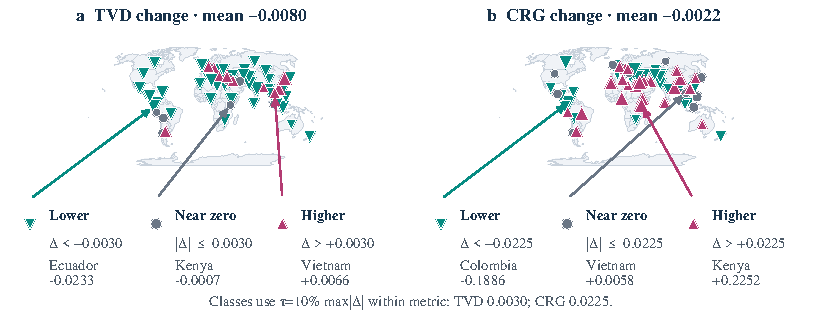
\includegraphics[width=\linewidth]{figs/figS4_country_maps.pdf}
  \caption{Country-level GPT-5.6-minus-GPT-5.5 changes in \textbf{a} TVD and \textbf{b}
  CRG. For each metric, lower, near-zero, and higher classes use
  $\tau=0.1\max|\Delta|$; external arrows locate three illustrative countries without
  obscuring the maps. Marker area tracks absolute magnitude. Countries are survey
  comparison units, and the patterns imply neither cultural homogeneity nor spatial
  diffusion.}
  \label{fig:country-maps-appendix}
\end{figure}
\FloatBarrier
